\subsection{Adversarial attacks on a trained system}

Attacks on trained systems are typically referred to as black-box or white-box. Black-box attacks are in the setting where the attackers do not know the trained neural network structure. A lot of research focus on the case where attackers are allowed to query the system and they aim to design a sequence of attacks that would find incorrect behaviour of the network in as few queries as possible. White-box attacks assume the attackers know and can exploit the neural network structure in some way. Some people also refer to grey-box attacks for the situation when there is partial knowledge available.

Training neural networks is expensive in terms of compute power. For a company like DSTL, they may consider off-loading the training process to an external company. This then raises a potential security issue of having external contractors with the knowledge of the neural network architecture. We therefore look at the white/grey-box settings.

The Fast Gradient Sign Method (FGSM) \cite{Goodfellow14} is an adversarial attack that adds a small perturbation \(\eta\):
\begin{equation}
\eta = \epsilon \text{sign}(\nabla_x J(\theta,x,y)),
\end{equation}
to the images. Where \(\theta\) are the parameters of the network, \(x\) are the input data, \(y\) are the targets and \(J(\theta,x,y)\) is the loss function used. Note that the required gradient is easily computed through backpropagation if the network structure is known (white-box).

\begin{figure}[h!]
	\centering
	\begin{subfigure}{.4\textwidth}
		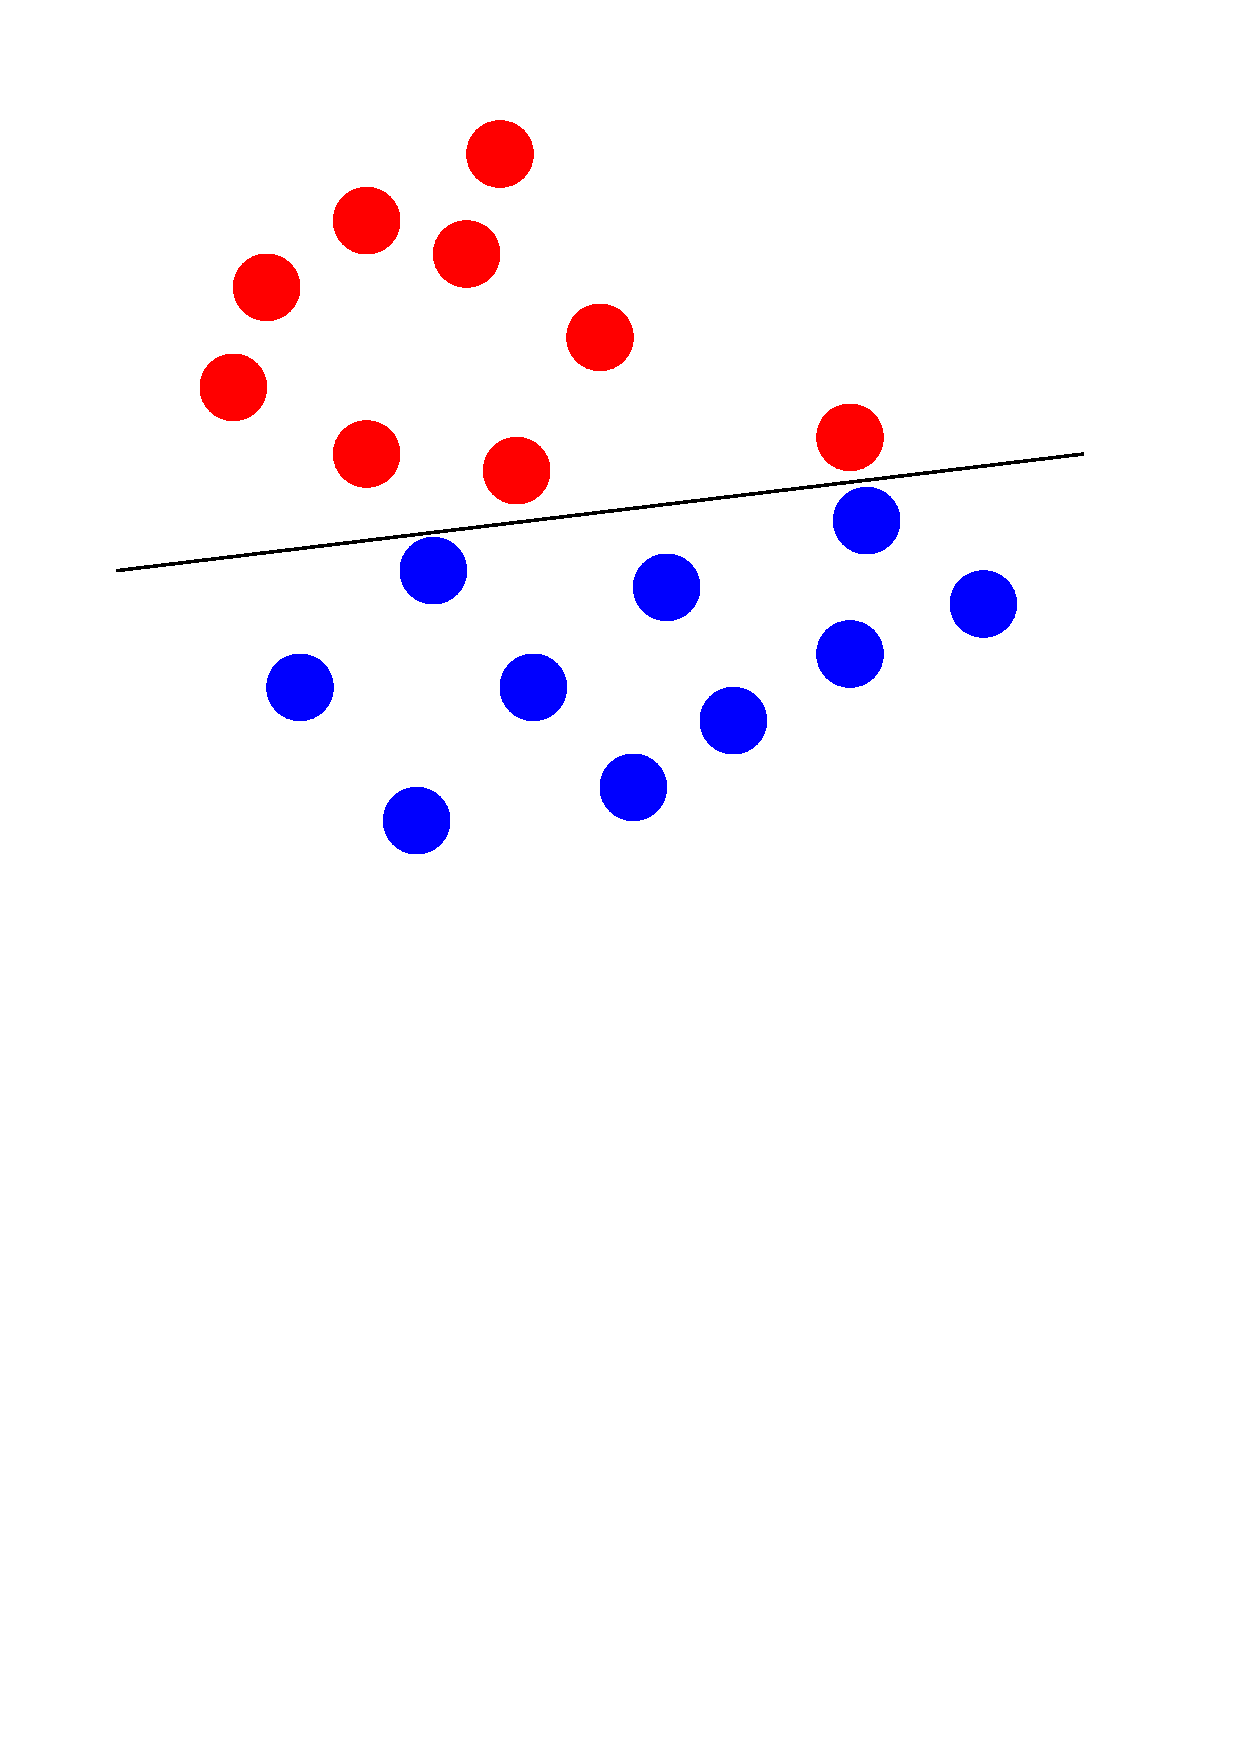
\includegraphics[width=\textwidth]{original}
		\caption{The original data}
		\label{fig:original}
	\end{subfigure}
	\begin{subfigure}{.4\textwidth}
		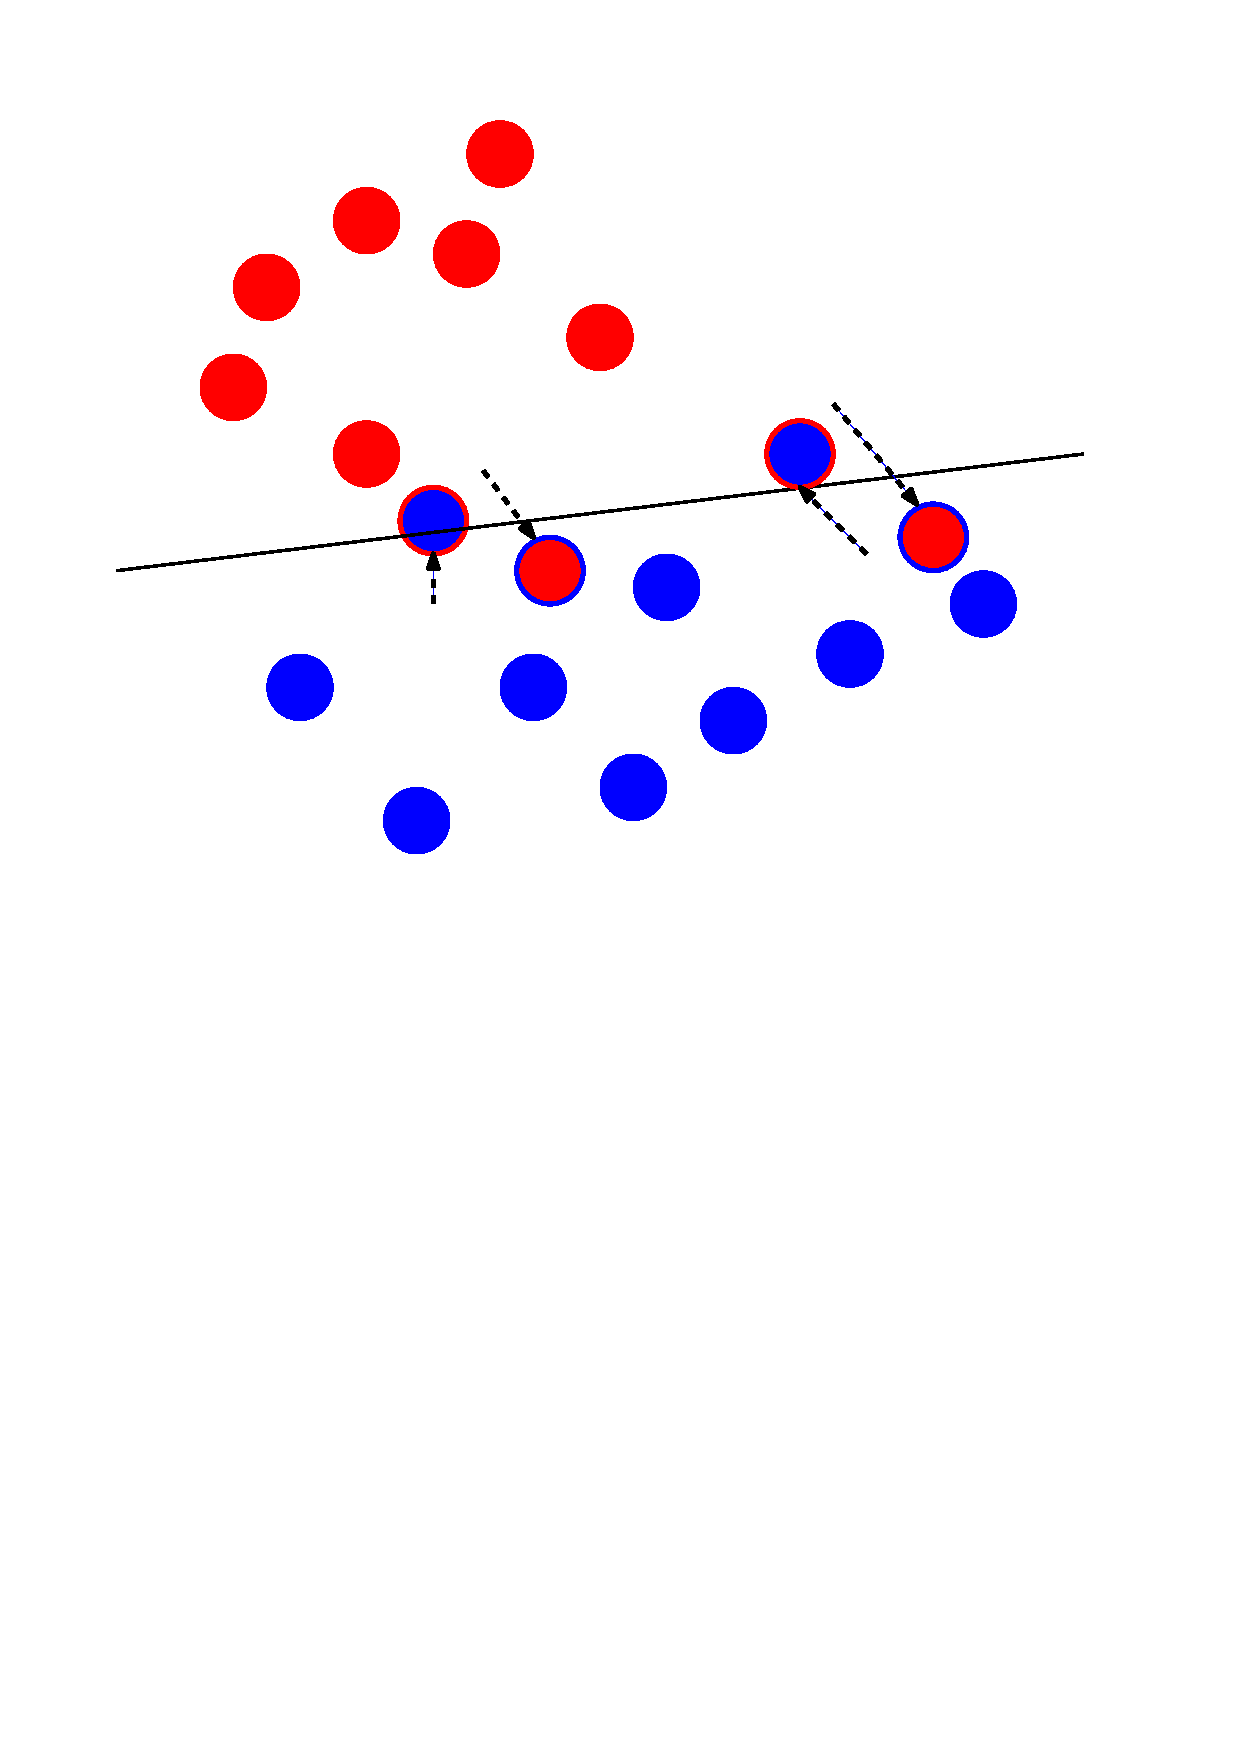
\includegraphics[width=\textwidth]{fgsm}
		\caption{Data with perturbations}
		\label{fig:fgsm}
	\end{subfigure}
	\caption{After perturbation.}
	\label{fig:fgsm_attack}
\end{figure}

Figure \ref{fig:fgsm_attack} gives a representation of a two dimensional, binary classification problem. A classifier should learn the optimal boundaries to split the two classes. In our case, this boundary is determined by the trained neural network and is depicted as a solid line in the figure. For attacks like the FGSM, the data is perturbed in a specific direction such that even a small perturbation will cause the data point to cross the classification boundary and become misclassified. As we can see on the right-hand side of the figure, perturbations have caused two red points and two blue points to cross the boundary, these would then be incorrectly classified.